\section{Dataset and Preprocessing}

\subsection*{Dataset}
We use the MVTec 3D-AD dataset, a benchmark designed for unsupervised 3D anomaly detection and localization \cite{bergmann2022mvtec3d}. The dataset is publicly available from the MVTec research page.\footnote{\url{https://www.mvtec.com/company/research/datasets/mvtec-3d-ad}} The current pipeline indexes all ten categories available in the local release: bagel, cable gland, carrot, cookie, dowel, foam, peach, potato, rope and tire.

The indexed data contain $4147$ samples in total. The training split contains $2656$ normal samples, the validation split contains $294$ normal samples and the test split contains $1197$ samples, of which $249$ are normal and $948$ are anomalous. Training and validation therefore preserve the unsupervised setting: no defective samples are used to fit the normality models.

\begin{figure*}[t]
    \centering
    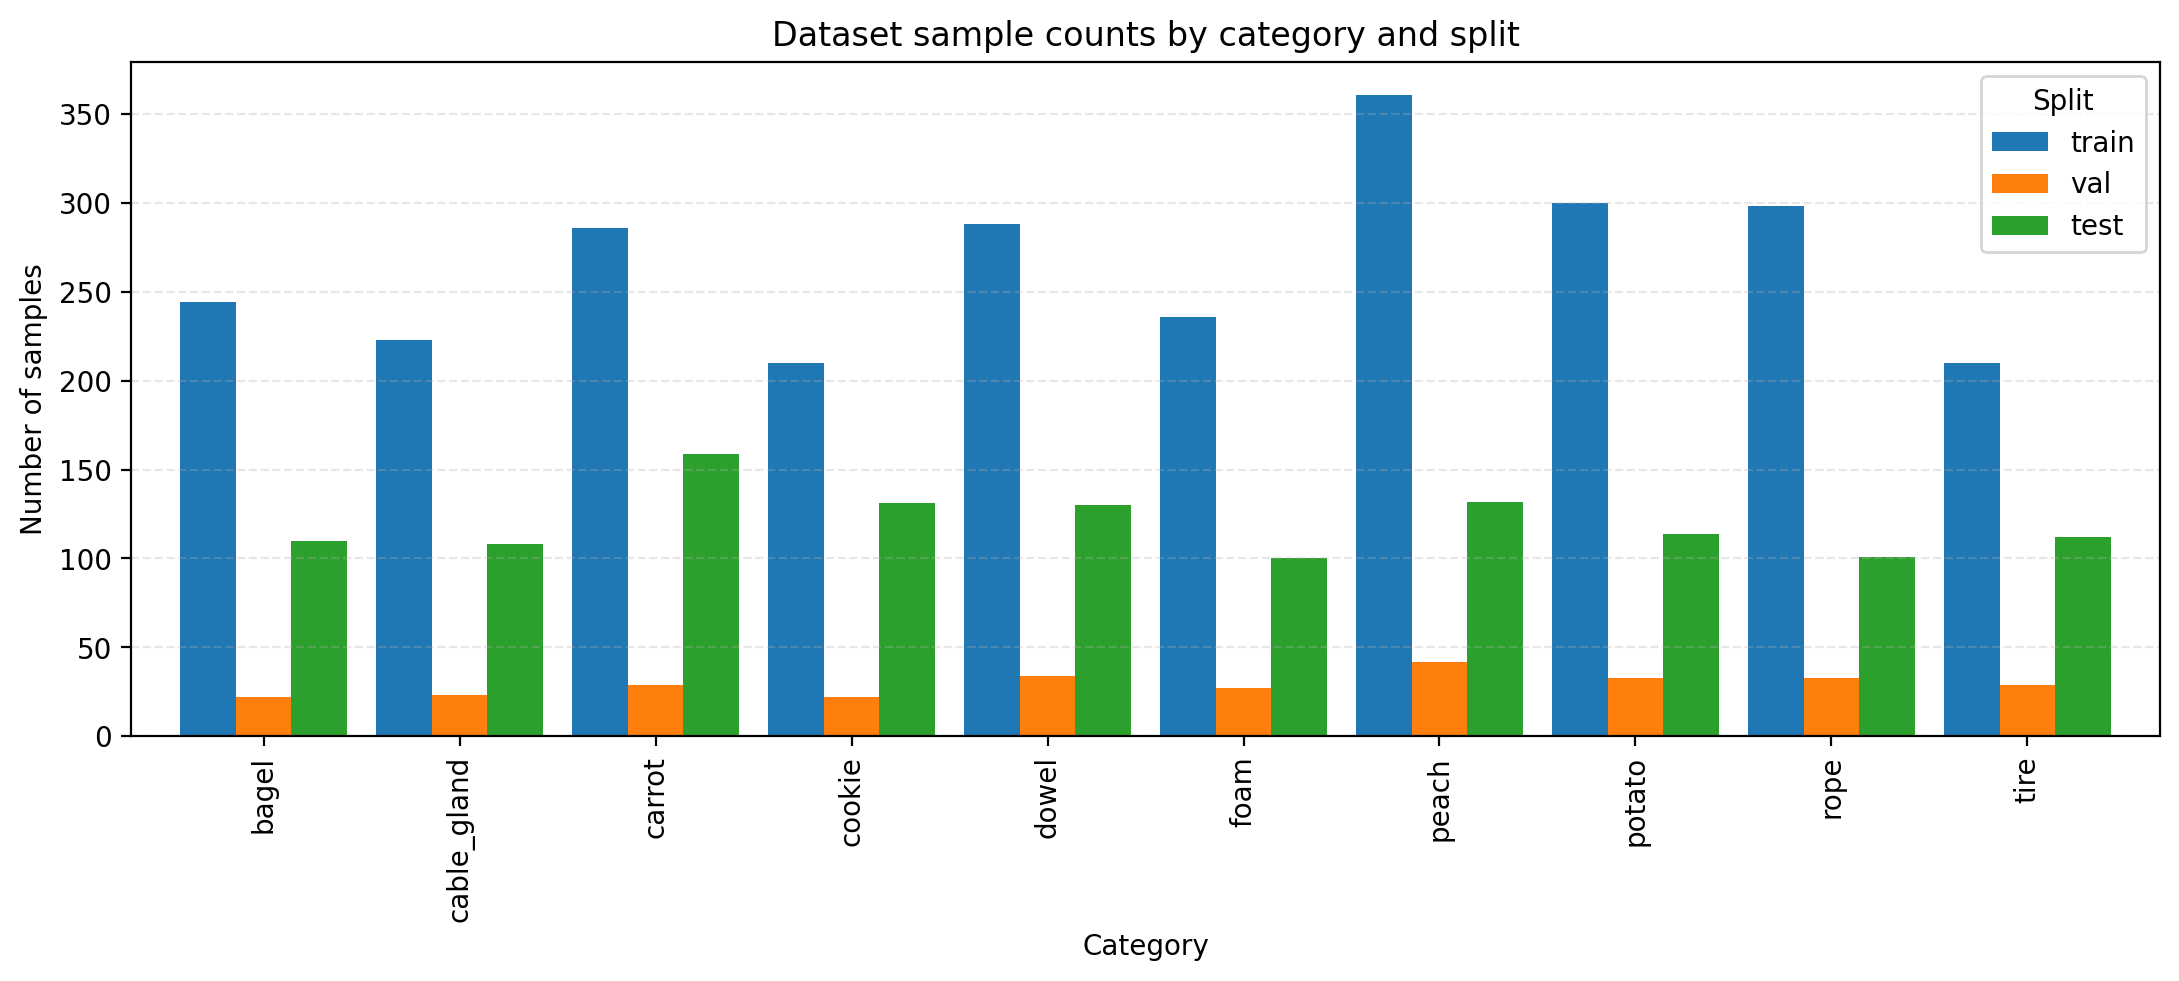
\includegraphics[width=0.92\textwidth]{figures/index_summary.png}
    \caption{Indexed MVTec 3D-AD samples by category, split and label.}
    \label{fig:index-summary}
\end{figure*}

\subsection*{Depth preprocessing}
The MVTec 3D-AD samples provide RGB images, XYZ point maps and ground-truth masks for defective test samples. The current shared representation is a depth map derived from the $Z$ channel of the raw XYZ file. Preprocessing performs valid-depth masking, foreground estimation, object cropping with a configurable margin, aspect-preserving resize, patch-grid snapping and per-image normalization over object pixels only. The processed output stores both the normalized depth map and a foreground mask.

The aspect-preserving resize is important because forcing all objects into a square canvas can introduce large empty areas and distort the patch raster. This was especially visible for elongated categories such as \textit{rope}. The final processed dimensions are snapped so that fixed-size patches land cleanly on image borders.

\begin{figure}[H]
    \centering
    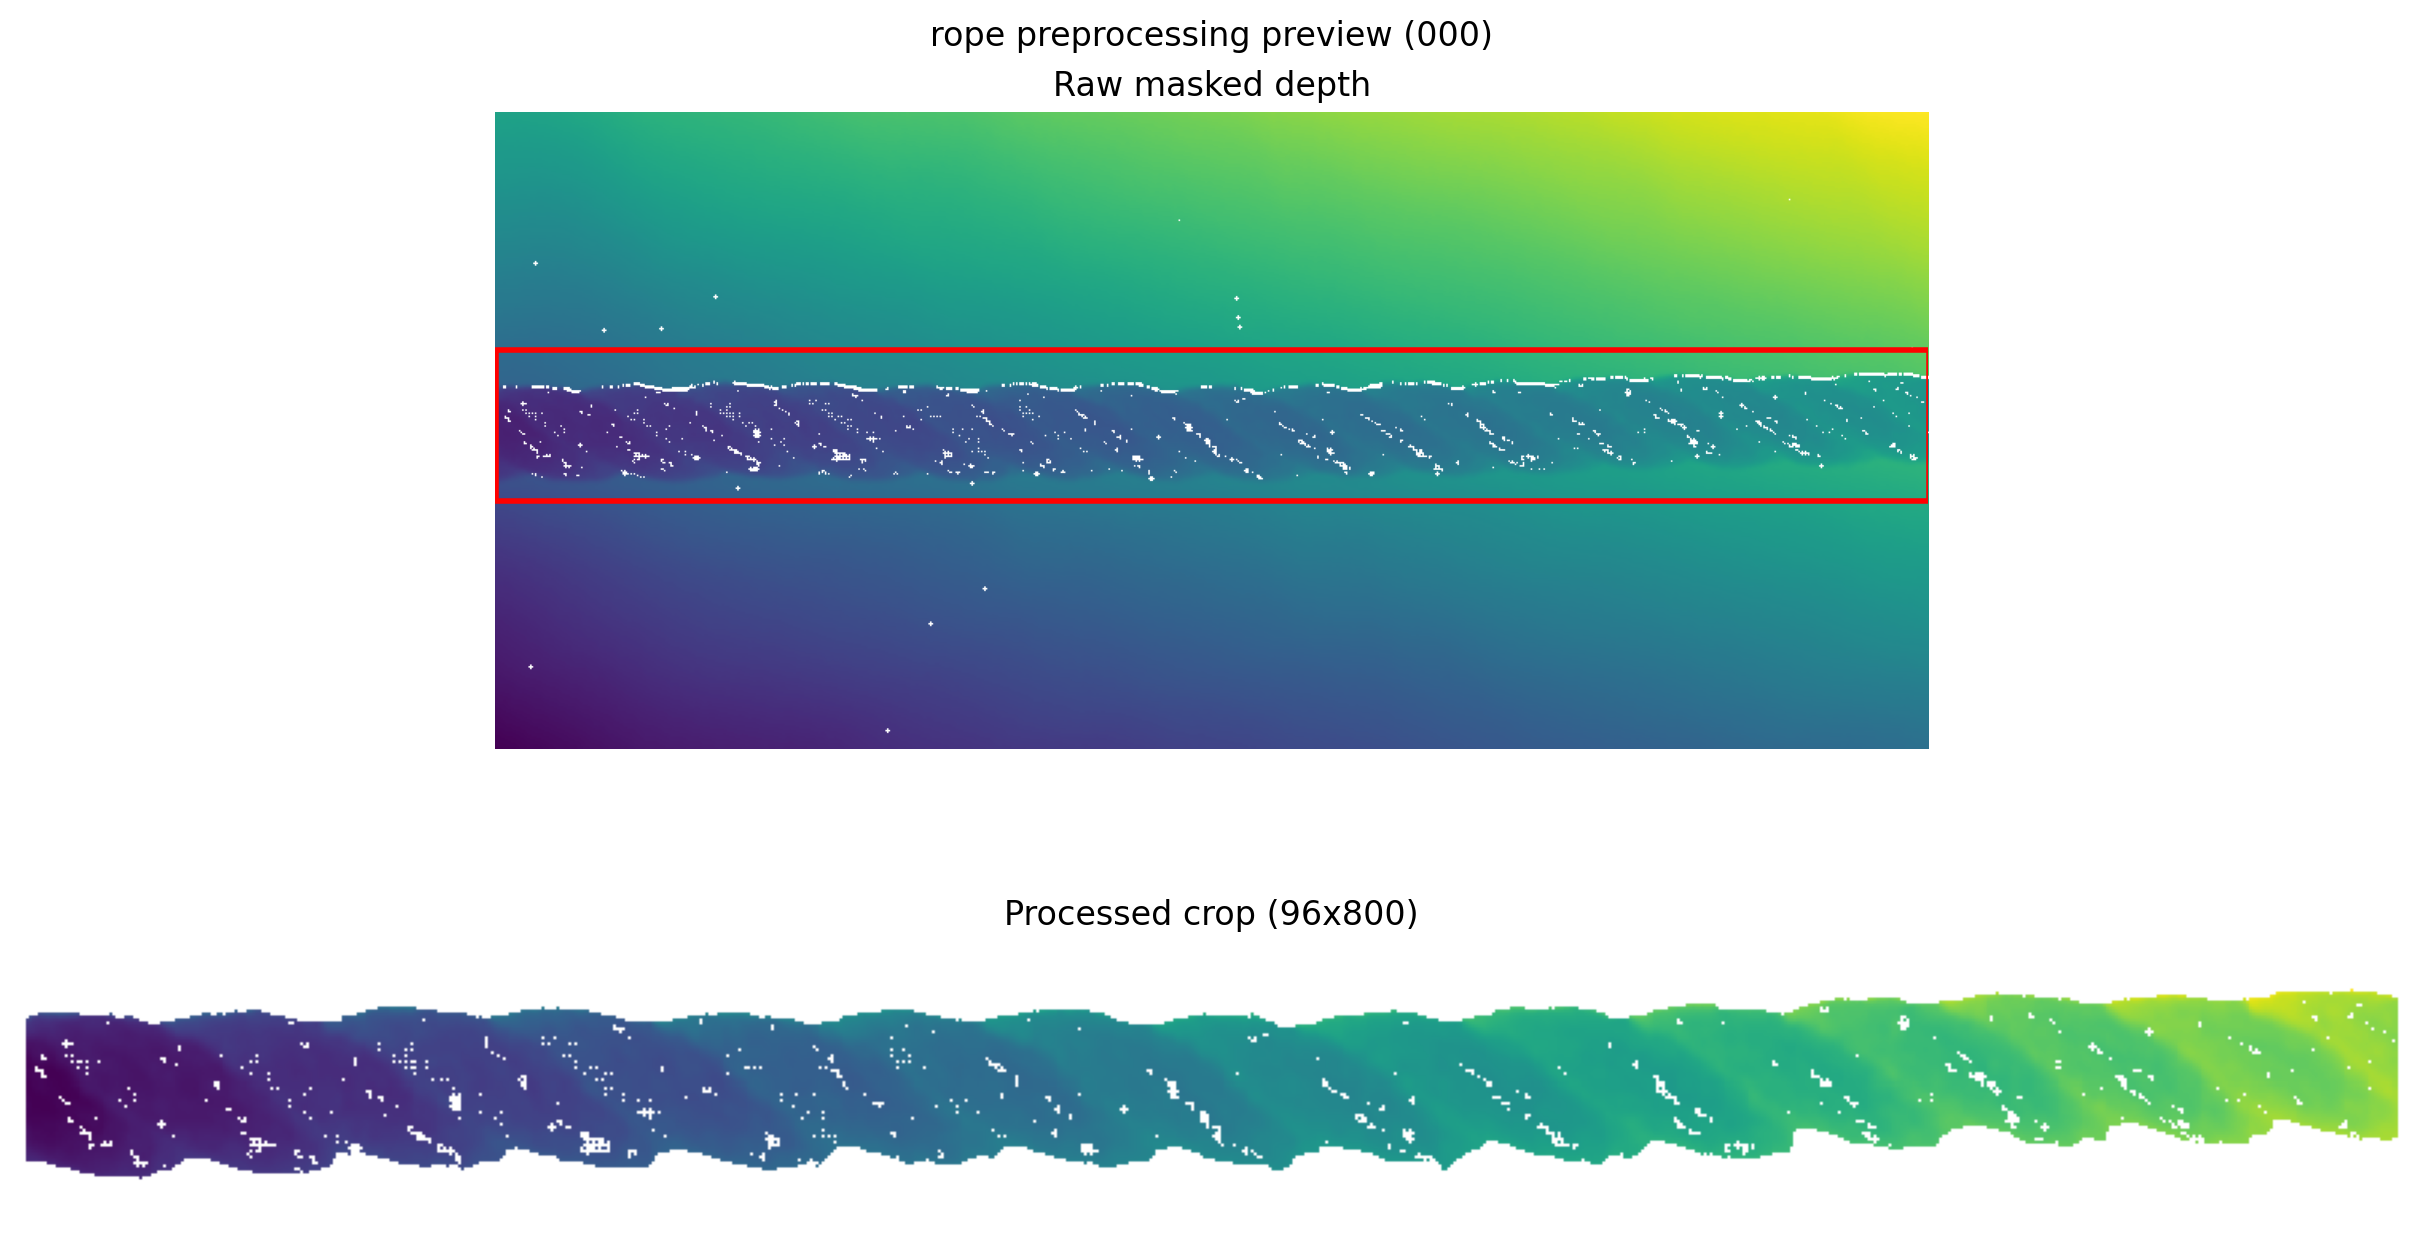
\includegraphics[width=\columnwidth]{figures/rope_raw_vs_processed.png}
    \caption{Example of the raw-to-processed depth transformation for an elongated object.}
    \label{fig:preprocessing-rope}
\end{figure}

\subsection*{Patch Extraction}
After preprocessing, each normalized depth map is divided into overlapping $32 \times 32$ local patches with stride $16 \times 16$. Patch coordinates are generated deterministically in row-major order. During training, patches with too little valid object area are skipped. During inference, patch scores are aggregated back to image space by averaging overlapping contributions. This patch-based representation increases the number of normal training examples and provides a direct route from local scores to anomaly heatmaps.
